% ============================================================================
% Appendix B --- Conceptual Extensions: Particles, Quantum, Classical
% From former Appendix B of Cosmochrony v1.13beta1, streamlined
% ============================================================================
\clearpage

\section{Conceptual Extensions of Cosmochrony ---
Particles, Quantum Phenomena, and Classical Limits}
\label{sec:appendix-conceptual}

This appendix illustrates how familiar particle, quantum, and classical
structures may emerge once the $\chi$ field admits localized and stable
configurations.
These developments serve as a conceptual bridge between the
mathematical foundations (Appendix~\ref{sec:appendix-math}) and the
cosmological considerations
(Appendix~\ref{sec:appendix-cosmo}).
None are required for the logical coherence of the framework.

% ----------------------------------------------------------------------------
% B.1 --- Interpretative Status of the chi Field
% From former B01, condensed
% ----------------------------------------------------------------------------
\subsection{Interpretative Status of the
\texorpdfstring{$\chi$}{χ} Field}
\label{subsec:nature-chi}

$\chi$ encodes a non-energetic relational scale of relaxation from
which duration, distance, and causal ordering are reconstructed.
The notation $\chi(x^\mu)$ is representational: spacetime coordinates
serve as labels for relational information in regimes where a stable
geometric description has emerged.
$\chi$ should not be interpreted as a matter field on spacetime, a
scalar coupled to a pre-existing metric, or a hidden-variable
replacement for the wavefunction.
Spacetime is an emergent bookkeeping structure \emph{for} $\chi$, not
a container \emph{of} $\chi$.

% ----------------------------------------------------------------------------
% B.2 --- Topological Configurations: Solitons as Particles
% From former B02, condensed
% ----------------------------------------------------------------------------
\subsection{Topological Configurations of the
\texorpdfstring{$\chi$}{χ} Field: Solitons as Particles}
\label{app:topological_solitons}

Solitonic configurations are effective geometric representations
illustrating how particle-like properties arise from stable, localized
configurations of $\chi_{\mathrm{eff}}$ once a smooth geometric
projection applies
(Appendix~\ref{app:relational_formulation}).

\subsubsection*{Charge as Oriented Relaxation Asymmetry}

A localized configuration deforms $\chi_{\mathrm{eff}}$ relative to
the background $\chi_{\mathrm{eff},0}$: excess (positive charge) or
deficit (negative charge).
The magnitude is diagnosed by a Gauss-like flux integral
$q_{\mathrm{eff}} \propto
  \oint_\Sigma \nabla\chi_{\mathrm{eff}} \cdot d\mathbf{S}$.
Coulomb-like interactions emerge from frustration minimization of the
Dirichlet functional
$\mathcal{F}[\chi_{\mathrm{eff}}]
  = \tfrac{1}{2}\int |\nabla\chi_{\mathrm{eff}}|^2\,d^3x$.

\begin{figure}[h]
  \centering
  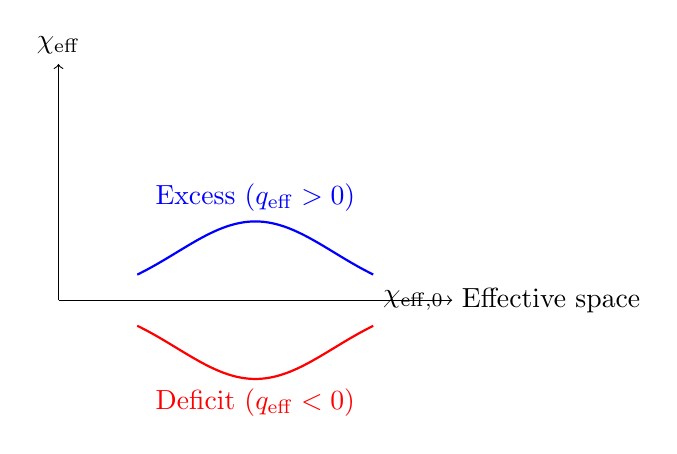
\begin{tikzpicture}[x=2cm, y=2cm]
    \draw[->] (0,0) -- (2.5,0)
      node[right] {Effective space};
    \draw[->] (0,0) -- (0,1.5)
      node[above] {$\chi_{\mathrm{eff}}$};
    \draw[thick, blue, domain=0.5:2, samples=100]
      plot (\x, {0.5*exp(-2*(\x-1.25)^2)});
    \node[blue, above] at (1.25, 0.5)
      {Excess ($q_{\mathrm{eff}}>0$)};
    \draw[thick, red, domain=0.5:2, samples=100]
      plot (\x, {-0.5*exp(-2*(\x-1.25)^2)});
    \node[red, below] at (1.25, -0.5)
      {Deficit ($q_{\mathrm{eff}}<0$)};
    \draw[dashed] (0.5,0) -- (2,0);
    \node[right] at (2,0)
      {$\chi_{\mathrm{eff},0}$};
  \end{tikzpicture}
  \caption{Oriented deformations of
    $\chi_{\mathrm{eff}}$ defining effective charge
    polarity.}
  \label{fig:chi_charges}
\end{figure}

\subsubsection*{Vortical Configurations and Integer-Spin
Excitations}
\label{subsec:vortices}

An effective winding number
$n = (2\pi)^{-1}
  \oint \nabla\arg(\chi_{\mathrm{eff}}) \cdot d\mathbf{l}$
characterizes charge orientation, topological robustness, and integer
spin.

\begin{figure}[h]
  \centering
  \begin{tikzpicture}[x=2cm, y=2cm]
    \draw[->] (-1.5,0) -- (1.5,0) node[right] {$x$};
    \draw[->] (0,-1.5) -- (0,1.5) node[above] {$y$};
    \foreach \r in {0.2,0.4,...,1.2} {
      \draw[blue, thick, domain=0:6.28, samples=100]
        plot ({\r*cos(\x)}, {\r*sin(\x)});
    }
    \fill[red] (0,0) circle (0.05);
    \node[red, below] at (0,0) {Core};
    \node[blue] at (1.2,1.2) {$n=1$};
  \end{tikzpicture}
  \caption{Vortical configuration with winding $n=1$
    (integer spin).}
  \label{fig:chi_vortex}
\end{figure}

\subsubsection*{Skyrmion-Like Configurations and
Spin-$\tfrac{1}{2}$ Excitations}
\label{subsec:skyrmions}

Configurations with topological index $Q = \pm 1$ exhibit
$4\pi$-periodicity under rotations, providing a geometric origin for
spin-$\tfrac{1}{2}$ behavior and fermionic statistics.

\begin{figure}[h]
  \centering
  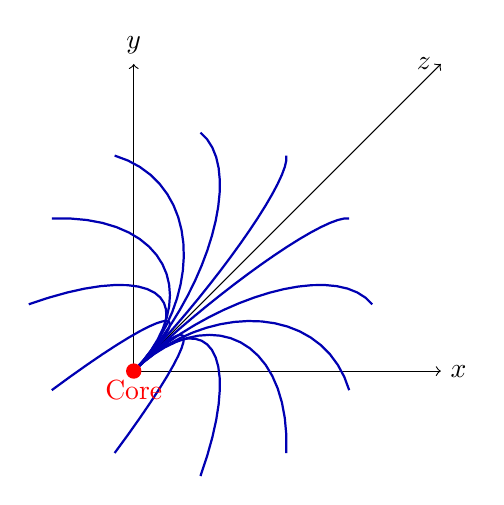
\begin{tikzpicture}[x=1.5cm, y=1.5cm, z=1.5cm,
    scale=1.3]
    \draw[->] (0,0,0) -- (2,0,0) node[right] {$x$};
    \draw[->] (0,0,0) -- (0,2,0) node[above] {$y$};
    \draw[->] (0,0,0) -- (0,0,2) node[left] {$z$};
    \foreach \phi in {0,30,...,330} {
      \draw[blue!70!black, thick,
        domain=0:1.2, samples=20]
        plot ({
          \x*sin(\x r)*cos(\phi)},
          {\x*sin(\x r)*sin(\phi)},
          {\x*cos(\x r)});
    }
    \fill[red] (0,0,0) circle (0.05);
    \node[red, below] at (0,0,0) {Core};
  \end{tikzpicture}
  \caption{Skyrmion-like configuration of
    $\chi_{\mathrm{eff}}$ (spin-$\tfrac{1}{2}$).}
  \label{fig:chi_skyrmion}
\end{figure}

\subsubsection*{Summary: Topology, Charge, and Spin}

\begin{table}[htbp]
  \centering
  \caption{Effective solitonic configurations and
    emergent particle properties.}
  \label{tab:solitons_charge}
  \begin{tabular}{|c|c|c|c|}
    \hline
    \textbf{Configuration} &
    \textbf{Index} &
    \textbf{$\chi_{\mathrm{eff}}$ asymmetry} &
    \textbf{Properties} \\
    \hline
    Vortical & $n$ &
    Excess/deficit &
    Charge $\propto n$, int.\ spin \\
    \hline
    Skyrmion & $Q=\pm 1$ &
    Oriented deformation &
    Charge $\propto Q$, spin-$\tfrac{1}{2}$ \\
    \hline
  \end{tabular}
\end{table}

\input{part6/appB/sec-soliton-energy-mass}
% ----------------------------------------------------------------------------
% B.4 --- 4pi-Periodic Soliton and Spinorial Behavior
% From former B04, condensed
% ----------------------------------------------------------------------------
\subsection{Example:
\texorpdfstring{$4\pi$}{4π}-Periodic Soliton and Spinorial
Behavior}
\label{subsec:4pi_soliton}

An illustrative construction supporting the topological interpretation
of spin
(Section~\ref{subsec:spin-statistics}).

In the projectable regime, certain localized excitations admit an
effective internal phase $\theta$.
A complex-valued proxy (the underlying field remains real):
$\chi_{\mathrm{eff}}(x)
  = \eta\tanh(\kappa x)\,e^{i\theta(x)}$.
Choosing $\theta(\alpha) = \alpha/2$:
\begin{equation}
  \psi(\alpha)
  \equiv \psi_0\,e^{i\alpha/2}.
  \label{eq:B4-half-angle-map}
\end{equation}
A $2\pi$ cycle inverts the sign:
\begin{equation}
  \psi(\alpha + 2\pi) = -\psi(\alpha).
  \label{eq:B4-2pi-sign}
\end{equation}
A $4\pi$ cycle restores identity:
\begin{equation}
  \psi(\alpha + 4\pi) = \psi(\alpha).
  \label{eq:B4-4pi-identity}
\end{equation}
Schematically:
\begin{equation}
  \begin{aligned}
    \alpha: 0 \to 2\pi
    &\Rightarrow \text{nontrivial loop }
      (\mathbb{Z}_2)
    \Rightarrow \psi \mapsto -\psi, \\
    \alpha: 0 \to 4\pi
    &\Rightarrow \text{trivial loop}
    \Rightarrow \psi \mapsto \psi.
  \end{aligned}
  \label{eq:B4-schematic-doublecover}
\end{equation}

This $4\pi$-periodicity mirrors the double-cover
$\mathrm{SU}(2) \to \mathrm{SO}(3)$ and provides a geometric basis
for fermion-like transformation behavior without fundamental spinor
fields.
The sign change is an effective encoding of the $\mathbb{Z}_2$
obstruction
(Section~\ref{subsec:status-formulation}:
$\pi_1(\mathcal{C}_{\mathrm{eff}}) = \mathbb{Z}_2$).

% ----------------------------------------------------------------------------
% B.5 --- Relation to Classical Limits
% From former B05, condensed
% ----------------------------------------------------------------------------
\subsection{Relation to Classical Limits}
\label{subsec:classical-limits}

Classical behavior corresponds to a dynamical regime where
$\chi_{\mathrm{eff}}$ varies slowly, localized excitations are dilute,
and topological constraints are suppressed.
Perturbations propagate as weak disturbances on an effectively flat
background, recovering superposition and approximate locality.
In the nonlinear regime, large gradients induce effective curvature and
horizon-like behavior.
The classical limit is defined not by $\hbar \to 0$ but by the
stability of a particular relaxation regime of the underlying~$\chi$
field.

\input{part6/appB/sec-status-formulation}
\input{part6/appB/sec-soliton-particle-solutions}
% ----------------------------------------------------------------------------
% B.8 --- Perspectives: Towards a Derivation of mp/me
% From former B08, condensed
% ----------------------------------------------------------------------------
\subsection{Perspectives: Towards a Derivation of the
Proton-to-Electron Mass Ratio}
\label{subsec:perspectives_mass_spectrum}

Normal modes of the stability operator
$\mathcal{L}_{\mathrm{sol}}\psi_n = \lambda_n\psi_n$ encode
intrinsic stiffness scales.
The effective mass scaling is
$m_n \propto \sqrt{\lambda_n}\,\chi_c$, and energy levels satisfy
$E_n \sim \lambda_n\chi_c^2$.

The proton is modeled as a composite three-soliton bound state
($Q = 3$, motivated by topological phase
locking~\cite{BattyeSutcliffe2022, MantonSutcliffe2004}), with
\[
  \frac{m_p}{m_e}
  \approx
  \sqrt{\frac{\lambda_{\mathrm{bind}}}{
    \lambda_e}},
  \quad
  \frac{\lambda_{\mathrm{bind}}}{\lambda_e}
  \sim 3.4 \times 10^6.
\]
The spectral packing fraction
$\alpha \equiv \lambda_e/\lambda_{\mathrm{bind}}
  \sim 3 \times 10^{-7}$
measures spectral compression from topological binding.
Heuristically,
$\lambda_{\mathrm{bind}}/\lambda_e
  \sim \chi_c^2$ gives $\chi_c \approx 8.3$.

\subsubsection*{Working Ansatz for $V(\chi)$}
\label{subsec:explicit_Vchi_ansatz}

A minimal two-scale effective potential:
\begin{equation}
  V(\chi)
  = \frac{\lambda}{4}
      (\chi^2 - \eta^2)^2
    + \varepsilon\,\eta^4
      \left[
        1 - \cos\!\left(
          \frac{\chi}{\eta}
        \right)
      \right],
  \label{eq:Vchi_multiwell_periodic}
\end{equation}
with $\varepsilon \ll 1$.

\subsubsection*{Linking $(\lambda,\eta)$ to Observables}
\label{subsec:lambda_eta_to_observables}

Dimensionless control combinations:
\begin{equation}
  g \equiv \lambda\,\chi_c^2\,\eta^2,
  \quad
  u \equiv \varepsilon.
  \label{eq:dimensionless_controls}
\end{equation}

\paragraph{Matching strategy.}
\label{matching-strategy-using-the-proton-to-electron-ratio}
The feasibility condition:
\begin{equation}
  \exists\,(g,u)
  \text{ s.t.}\quad
  \frac{\lambda_{\mathrm{bind}}(Q{=}3;\,g,u)}
       {\lambda_e(g,u)}
  \approx 3.4 \times 10^6,
  \label{eq:feasibility_condition_lambda_eta}
\end{equation}
while remaining stable under small $(g,u)$ variations.

\subsubsection*{Numerical Program}
\label{subsec:numerical_program_mass_ratio}

The pipeline tests whether bounded relaxation plus
$V(\chi)$ admits stable sectors with
$\lambda_{\mathrm{bind}}/\lambda_e \sim 10^6$ without fine-tuning:
dynamics and formation, soliton harvesting by topological
classification, stability operator extraction, spectral ratio test,
and fine-structure diagnostics.

% ----------------------------------------------------------------------------
% B.9 --- Spectral Scaling and the Projection Ontology
% From former B09, condensed
% ----------------------------------------------------------------------------
\subsection{Spectral Scaling and the Projection Ontology}
\label{subsec:spectral-scaling-projection-ontology}

Inertial mass is a spectral signature of projection visibility.
The non-injective projection $\Pi$ implies that each effective particle
corresponds to a large equivalence class of micro-configurations whose
stability eigenvalues measure the fiber weight.
The ratio
$m_p/m_e \approx \sqrt{\lambda_p/\lambda_e}$
is independent of the absolute action scale $\hbar_\chi$ and is
therefore a structurally protected invariant.

\begin{figure}[htbp]
  \centering
  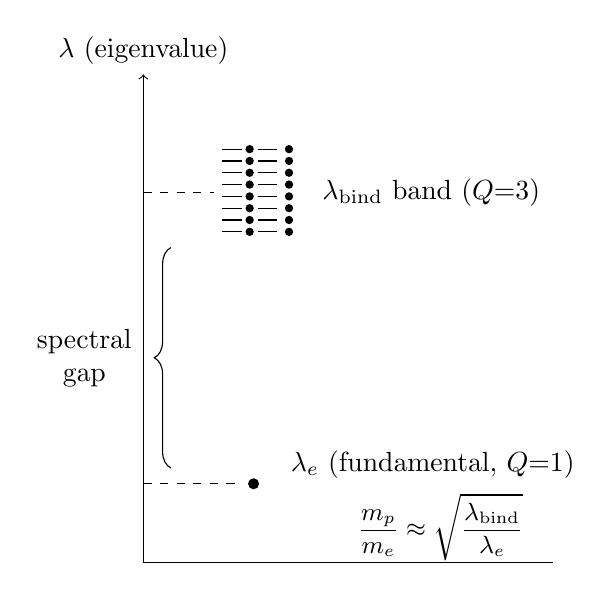
\begin{tikzpicture}[x=1cm,y=1cm]
    \draw[->] (0,0) -- (0,6.2)
      node[above] {$\lambda$ (eigenvalue)};
    \draw (0,0) -- (5.2,0);
    \fill (1.4,1.0) circle (2pt);
    \node[anchor=west] at (1.75,1.25)
      {$\lambda_e$ (fundamental, $Q{=}1$)};
    \foreach \y in
      {4.2,4.35,4.5,4.65,4.8,4.95,5.1,5.25} {
      \draw (1.0,\y) -- (1.25,\y);
      \fill (1.35,\y) circle (1.5pt);
      \draw (1.45,\y) -- (1.70,\y);
      \fill (1.85,\y) circle (1.5pt);
    }
    \node[anchor=west] at (2.15,4.7)
      {$\lambda_{\mathrm{bind}}$ band ($Q{=}3$)};
    \draw[decorate,
      decoration={brace,amplitude=6pt}]
      (0.35,1.2) -- (0.35,4.0)
      node[midway,xshift=-1.1cm,align=center]
        {spectral\\gap};
    \draw[dashed] (0,1.0) -- (1.2,1.0);
    \draw[dashed] (0,4.7) -- (0.9,4.7);
    \node[anchor=west,align=left] at (2.6,0.45)
      {\small $\displaystyle
        \frac{m_p}{m_e}
        \approx
        \sqrt{\frac{\lambda_{\mathrm{bind}}}
                   {\lambda_e}}$};
  \end{tikzpicture}
  \caption{Spectral gap in the stability spectrum of
    $\mathcal{L}_{\mathrm{sol}}$: elementary mode
    $\lambda_e$ separated from binding-mode band
    $\lambda_{\mathrm{bind}}$.}
  \label{fig:spectral-gap}
\end{figure}

% ----------------------------------------------------------------------------
% B.10 --- Spectral Characterization of Mass
% From former B10, condensed
% ----------------------------------------------------------------------------
\subsection{Spectral Characterization of Mass and the Secondary
Role of \texorpdfstring{$V(\chi)$}{V(χ)}}
\label{subsec:spectral_mass}

Particle masses emerge as eigenmodes of an effective relaxation
operator $\Delta_G^{(0)}\psi_n = -\lambda_n\psi_n$, with
$m_n c^2 \propto \sqrt{\lambda_n}\,\chi_c$.
This is analogous to bounded elastic systems where vibrational
frequencies arise from geometry and connectivity.

Three conceptual levels are distinguished: the background-independent
spectral operator (fundamental), coarse-grained
$\chi_{\mathrm{eff}}$ geometry (emergent), and interaction-induced
redistributions (dynamical).
$V(\chi)$ plays a secondary role, providing local stabilization and
fine splittings without setting the overall mass scale.
Its admissible form is constrained by compatibility with the
pre-existing spectral structure.
Potential-induced corrections shift eigenvalues as
$\lambda_n \to \lambda_n^{(0)} + \Delta\lambda_n^{(V)}$, affecting
small splittings (e.g.\ neutron--proton) while leaving topologically
dominated ratios largely invariant.

\input{part6/appB/sec-hbar-eff}
\input{part6/appB/sec-renormalization}
% ----------------------------------------------------------------------------
% B.13 --- Structural Origin of Quantum Correlations
% From former B13, condensed
% ----------------------------------------------------------------------------
\subsection{Structural Origin of Quantum Correlations and
Non-Locality}
\label{app:structural-origin-quantum-correlations}

The non-injective projection $\Pi$ provides a structural
reinterpretation: what appear as two spatially separated particles may
correspond to a single relational configuration in $\chi$.
Entanglement is the manifestation of a single $\chi$-source through
multiple non-injective projective images.
Spin correlations arise from torsional conservation: a local
stabilization at~$A$ structurally constrains admissible projective
states at~$B$ originating from the same source.
Bell inequality violations are attributed to the use of emergent
metric locality in a context where correlations are established prior
to spacetime separation.
The framework remains ontologically realist at the substrate level but
structurally non-local with respect to the emergent spacetime.

% ----------------------------------------------------------------------------
% B.14 --- Metastability, Decay Channels, Exponential Lifetimes
% From former B14, condensed
% ----------------------------------------------------------------------------
\subsection{Metastability, Decay Channels, and Exponential
Lifetimes}
\label{subsec:metastability-decay-channels-and-exponential-lifetimes}

\subsubsection*{Diagnostic Structural Functional}
\label{subsec:diagnostic-structural-functional}

$E_{\mathrm{struct}}[\chi_{\mathrm{eff}}]
  \sim \int_\mathcal{V}
    (|\nabla\chi_{\mathrm{eff}}|^2
     + \mu^2|\chi_{\mathrm{eff}}|^2)\,d^3x$
quantifies resistance to relaxation.

\subsubsection*{Admissible Factorization Channels}
\label{subsec:admissible-factorization-channels}

A decay channel is an admissible factorization preserving topological
invariants:
$Q(\chi_{\mathrm{eff},A})
  = \sum_i Q(\chi_{\mathrm{eff},i})$.
Kinematic accessibility requires
$\Delta E_{\mathrm{struct}} > 0$.
The survival probability is
$P(\tau) = \exp(-\Gamma\tau)$ with
$\Gamma = \sum_c \Gamma_c$.

Different interaction classes correspond to different degrees of
constraint: strong decays involve direct topological reorganization,
electromagnetic decays preserve core topology, and weak decays require
deep reconfiguration through rarer paths.

\subsubsection*{Non-Injective Projection and Structural
Factorization}
\label{subsec:non-injective-projection-and-structural-factorization}

Entanglement: a single $\chi_0$ admits a non-factorizable projection.
Decay: the projection becomes unstable and admissibility is recovered
through factorization
$\Pi(\chi_0) \to
  \Pi(\chi_1) \oplus \Pi(\chi_2) \oplus \cdots$.
The distinction is not at the substrate level but in the stability
properties of the projected description.

\input{part6/appB/sec-measurement-antiparticles}
% ----------------------------------------------------------------------------
% B.16 --- Structural Interpretation of CPT Symmetry
% From former B16, condensed
% ----------------------------------------------------------------------------
\subsection{Structural Interpretation of CPT Symmetry}
\label{subsec:structural-interpretation-of-cpt-symmetry}

The combined transformation
$(Q,\tau,\mathbf{x}) \to (-Q,-\tau,-\mathbf{x})$
leaves admissibility conditions invariant.
Under factorization, conservation of signed invariants enforces
particle--antiparticle pairs.
CPT symmetry emerges as an invariance of the admissible projection
structure.

\begin{figure}[t]
  \centering
  \begin{tikzpicture}[
    box/.style={draw, rounded corners,
      align=center, inner sep=6pt},
    arr/.style={->, thick},
    lab/.style={font=\small, align=center}]
    \node[box] (chi)
      {$\chi$\\[-2pt]
       \footnotesize relational config.};
    \node[box, below=1.6cm of chi] (proj)
      {$\Pi(\chi)$\\[-2pt]
       \footnotesize non-injective};
    \node[box, below left=2.2cm and 2.4cm of proj]
      (ent) {Entanglement\\[-2pt]
        \footnotesize non-factorizable};
    \node[box, below=2.2cm of proj]
      (meas) {Measurement\\[-2pt]
        \footnotesize selection};
    \node[box, below right=2.2cm and 2.4cm of proj]
      (dec) {Decay\\[-2pt]
        \footnotesize factorization};
    \node[box, below=1.8cm of dec, xshift=-2cm]
      (p) {Particle\\[-2pt]
        \footnotesize $+Q$};
    \node[box, below=1.8cm of dec, xshift=0cm]
      (ap) {Antiparticle\\[-2pt]
        \footnotesize $-Q$};
    \node[box, below=1.8cm of dec, xshift=2cm]
      (rad) {Light modes};
    \draw[arr] (chi)
      -- node[lab, right] {projection} (proj);
    \draw[arr] (proj) -- (ent);
    \draw[arr] (proj) -- (meas);
    \draw[arr] (proj) -- (dec);
    \draw[arr] (dec) -- (p);
    \draw[arr] (dec) -- (ap);
    \draw[arr] (dec) -- (rad);
  \end{tikzpicture}
  \caption{Unified structural interpretation:
    entanglement, measurement, and decay all originate
    from $\Pi$.
    Antiparticles emerge when signed invariants are
    redistributed.}
  \label{fig:projection-entanglement-decay}
\end{figure}

\input{part6/appB/sec-cp-asymmetry}
